% Inside the branch unit of the BTB design (designs/dualissue-btb/branchunit.v):
% lane selection, resolution (one comparator, one adder), check of the prediction and
% the signals that update the BTB.
\documentclass[tikz,border=3mm]{standalone}
\usepackage{xfp}
\usepackage[T1]{fontenc}
\usepackage{tgheros}
\renewcommand{\familydefault}{\sfdefault}
% Shared TikZ helpers for the datapath figures (Harris & Harris style, ch. 7.5).
%   32-bit buses: thick black; narrow fields (Rs/Rd): thin black;
%   control / hazard signals: thin blue; additions of the dual-issue design: green.
\usetikzlibrary{calc}
\usetikzlibrary{circuits.logic.US}

\definecolor{ctl}{RGB}{11,111,184}    % control unit / hazard unit (blue, as in the book)
\definecolor{new}{RGB}{21,128,61}     % elements added for the dual-issue design
\definecolor{hzd}{RGB}{217,95,2}     % hazard unit and its wires (orange)
\definecolor{bru}{RGB}{124,58,237}   % shared branch unit (purple)

\tikzset{
  w/.style   = {line width=1.1pt},               % 32-bit datapath wire
  nw/.style  = {line width=0.45pt},              % narrow datapath field (5 bits)
  c/.style   = {line width=0.45pt, ctl},         % control wire
  n/.style   = {line width=0.45pt, new},         % dual-issue control wire
  h/.style   = {line width=0.45pt, hzd},         % hazard unit wire
  blk/.style = {line width=1.1pt, fill=white},
  lab/.style = {font=\fontsize{6.5}{6.5}\selectfont, inner sep=1pt},
  bit/.style = {font=\fontsize{5}{5}\selectfont, inner sep=0.6pt},
  mxl/.style = {font=\fontsize{4.3}{4.3}\selectfont, inner sep=0.4pt},
  ttl/.style = {font=\fontsize{7.5}{7.5}\selectfont\bfseries, inner sep=1pt, align=center},
}

% wire junction (T joints)
\newcommand{\dotat}[1]{\fill #1 circle (0.045);}

% \Mux[labels]{name}{x}{yc}{n}{d}{s}
%   vertical n:1 multiplexer pointing right, inputs spaced d.
%   s = +1: input 0 is the lowest one; s = -1: input 0 is the highest one.
%   labels: optional comma list written inside (default 0..n-1).
%   anchors: name-0 .. name-(n-1), name-o (output),
%            name-t / name-b (select, top / bottom),
%            name-so / name-si (select on the side of the last / first input)
\newcommand{\muxhw}{0.2}
\newcommand{\Mux}[7][]{%
  \pgfmathsetmacro\mh{(#5*#6+0.2)/2}%
  \draw[blk] (#3-\muxhw,#4-\mh) -- (#3-\muxhw,#4+\mh) -- (#3+\muxhw,#4+\mh-0.13)
             -- (#3+\muxhw,#4-\mh+0.13) -- cycle;
  \pgfmathtruncatemacro\mlast{#5-1}%
  \foreach \i in {0,...,\mlast} {
    \pgfmathsetmacro\my{#4 + #7*(\i-(#5-1)/2)*#6}
    \coordinate (#2-\i) at (#3-\muxhw,\my);
  }
  \def\mlabs{#1}%
  \ifx\mlabs\empty
    \foreach \i in {0,...,\mlast} {
      \node[mxl, anchor=west] at ($(#2-\i)+(0.02,0)$) {\i};
    }
  \else
    \foreach \lb [count=\i from 0] in {#1} {
      \node[mxl, anchor=west] at ($(#2-\i)+(0.02,0)$) {\lb};
    }
  \fi
  \coordinate (#2-o) at (#3+\muxhw,#4);
  \coordinate (#2-t) at (#3,#4+\mh-0.065);
  \coordinate (#2-b) at (#3,#4-\mh+0.065);
  \coordinate (#2-so) at (#3,#4+#7*\mh-#7*0.065);
  \coordinate (#2-si) at (#3,#4-#7*\mh+#7*0.065);
}

% \Alu{name}{x}{ylo}{yhi}{text}: ALU / adder shape (chevron with notch),
%   output name-o; text is written horizontally (use \AluV for a rotated "ALU")
\newcommand{\AluShape}[4]{%
  \pgfmathsetmacro\ac{(#3+#4)/2}\pgfmathsetmacro\ah{#4-#3}%
  \draw[blk] (#2,#3) -- (#2+0.9,#3+0.25*\ah) -- (#2+0.9,#4-0.25*\ah) -- (#2,#4)
             -- (#2,\ac+0.12*\ah) -- (#2+0.2,\ac) -- (#2,\ac-0.12*\ah) -- cycle;
  \coordinate (#1-o) at (#2+0.9,\ac);
}
\newcommand{\Alu}[5]{%
  \AluShape{#1}{#2}{#3}{#4}%
  \node[lab, font=\fontsize{7}{7}\selectfont\bfseries] at (#2+0.58,\ac) {#5};
}
\newcommand{\AluV}[5]{%
  \AluShape{#1}{#2}{#3}{#4}%
  \node[lab, font=\fontsize{8}{8}\selectfont, rotate=90] at (#2+0.6,\ac) {#5};
}

% \PipeReg{x}{yin}{ymid}{yout}{note}: pipeline register of one lane.
%   yin = edge next to the middle of the figure, yout = outer edge (clock side),
%   ymid = boundary between the datapath part (black) and the control part (blue).
%   As in the book the clock is always on the top edge (labelled CLK only when the
%   top edge is the outer one) and the note (e.g. CLR) is written at the bottom edge,
%   where the hazard unit signal comes in.
\newcommand{\PipeReg}[5]{%
  \draw[blk] (#1-0.175,#2) rectangle (#1+0.175,#3);
  \draw[line width=1.1pt, ctl, fill=white] (#1-0.175,#3) rectangle (#1+0.175,#4);
  \pgfmathsetmacro\pt{max(#2,#4)}\pgfmathsetmacro\pb{min(#2,#4)}%
  \draw[line width=0.5pt] (#1-0.12,\pt) -- (#1,\pt-0.15) -- (#1+0.12,\pt);
  \ifdim #4pt>#2pt \node[lab, anchor=south] at (#1,\pt+0.05) {CLK};\fi
  \node[bit, rotate=90, anchor=center] at (#1,\pb+0.3) {#5};
}

% \Bar{x}{ylo}{yhi}: plain register (clock on the top edge)
\newcommand{\Bar}[3]{%
  \pgfmathsetmacro\bt{max(#2,#3)}%
  \draw[blk] (#1-0.175,#2) rectangle (#1+0.175,#3);
  \draw[line width=0.5pt] (#1-0.12,\bt) -- (#1,\bt-0.15) -- (#1+0.12,\bt);
}

\definecolor{opt}{RGB}{139,90,43}
\tikzset{o/.style = {line width=0.45pt, opt}}
\usetikzlibrary{decorations.pathreplacing}
\newcommand{\sigk}[2]{\textit{#1}\textsubscript{#2}}
\begin{document}
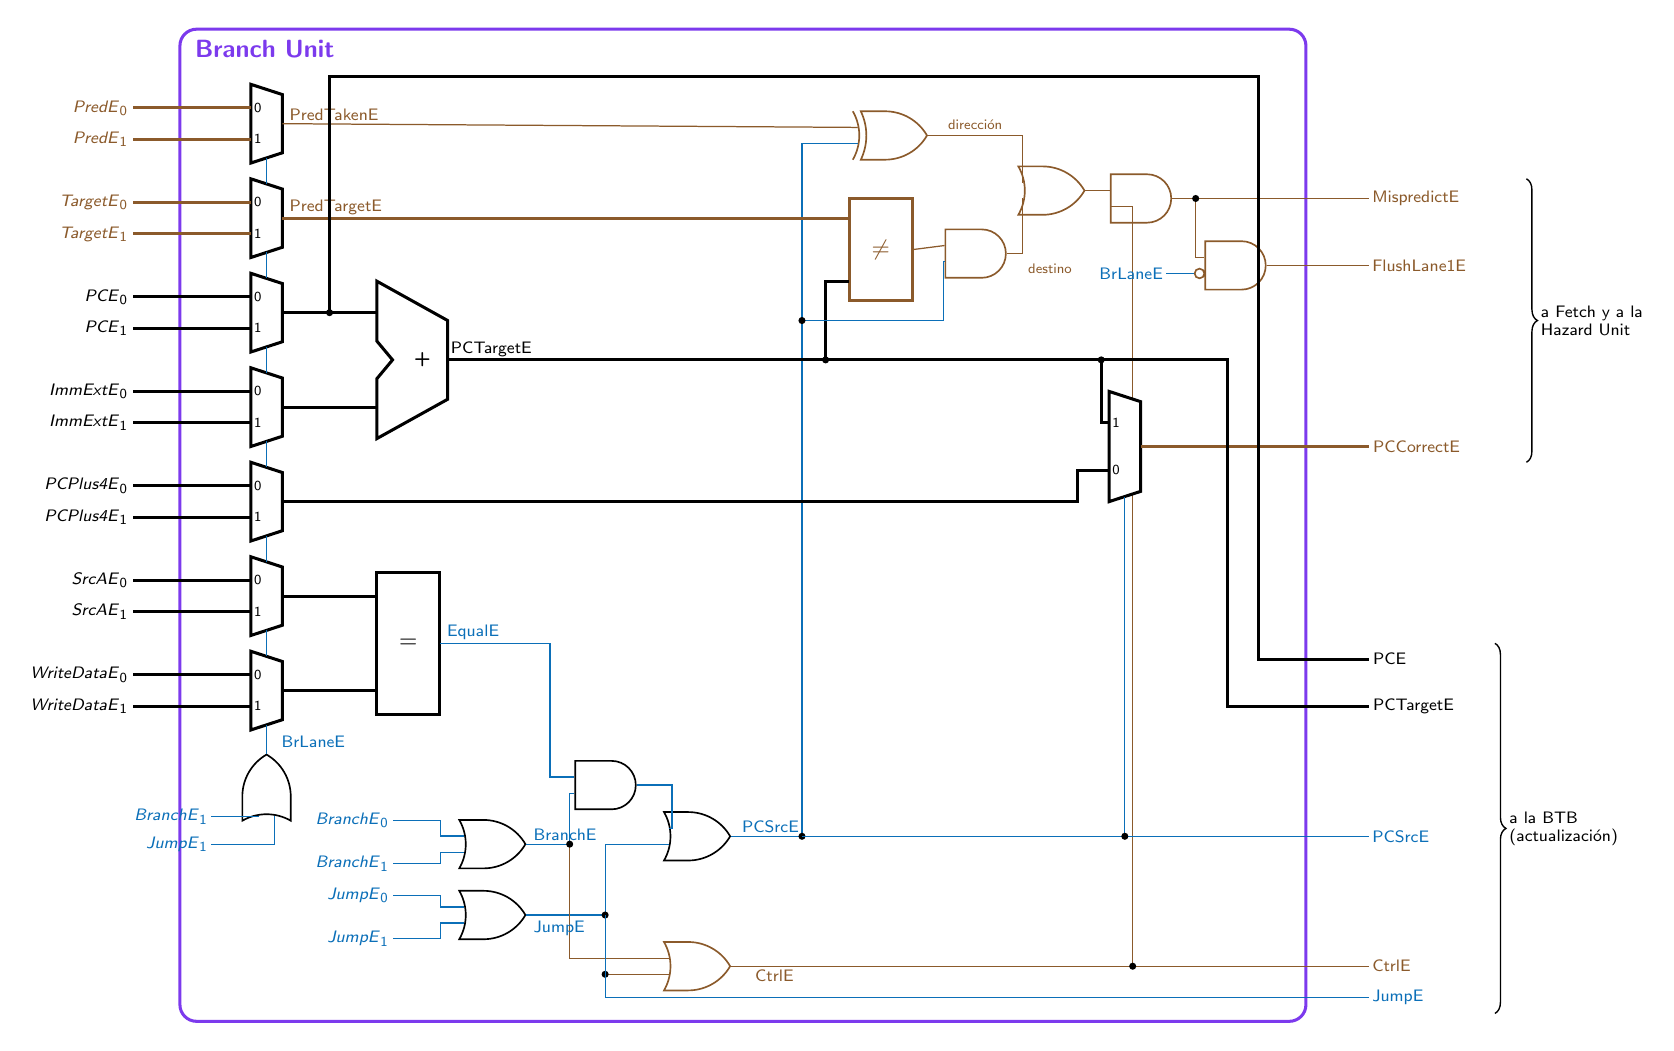
\begin{tikzpicture}[x=1cm,y=1cm, circuit logic US, medium circuit symbols,
  every circuit symbol/.style={line width=0.6pt, fill=white}]
% unit boundary
\draw[line width=1.1pt, bru, rounded corners=6pt] (0.9,-3.0) rectangle (15.2,9.6);
\node[lab, bru, font=\fontsize{9}{9}\selectfont\bfseries, anchor=north west] at (1.05,9.5) {Branch Unit};

% ---------------- lane selection: BrLaneE = BranchE_1 + JumpE_1 ----------------
% rows: Pred 8.4, Target 7.2, PC 6.0, Imm 4.8, PCPlus4 3.6, SrcA 2.4, SrcB (rs2) 1.2
\foreach \nm/\y/\a/\b/\isopt in {pd/8.4/PredE/PredE/1, tg/7.2/TargetE/TargetE/1, pc/6.0/PCE/PCE/0,
                                 im/4.8/ImmExtE/ImmExtE/0, p4/3.6/PCPlus4E/PCPlus4E/0,
                                 sa/2.4/SrcAE/SrcAE/0, sb/1.2/WriteDataE/WriteDataE/0} {
  \Mux{\nm}{2.0}{\y}{2}{0.4}{-1}
  \ifnum\isopt=1 \def\cl{opt}\else \def\cl{black}\fi
  \draw[w, \cl] (\nm-0) -- (0.3,0 |- \nm-0) node[lab, \cl, anchor=east] {\sigk{\a}{0}};
  \draw[w, \cl] (\nm-1) -- (0.3,0 |- \nm-1) node[lab, \cl, anchor=east] {\sigk{\b}{1}};
}
\draw[o] (pd-0) -- (0.3,0 |- pd-0);  \draw[o] (pd-1) -- (0.3,0 |- pd-1);   % 1-bit prediction
\foreach \a/\b in {pd/tg, tg/pc, pc/im, im/p4, p4/sa, sa/sb} \draw[c] (\a-b) -- (\b-t);
\node[or gate, inputs=nn, rotate=90, anchor=output] (gl) at (2.0,0.4) {};
\draw[c] (gl.output) -- (sb-b);
\draw[c] (gl.input 1) |- (1.3,-0.4) node[lab, ctl, anchor=east] {\sigk{BranchE}{1}};
\draw[c] (gl.input 2) |- (1.3,-0.75) node[lab, ctl, anchor=east] {\sigk{JumpE}{1}};
\node[lab, ctl, anchor=west] at (2.15,0.55) {BrLaneE};

% ---------------- resolution ----------------
\Alu{add}{3.4}{4.4}{6.4}{+}
\draw[w] (pc-o) -- (3.4,6.0);
\draw[w] (im-o) -- (3.4,4.8);
\draw[blk] (3.4,0.9) rectangle (4.2,2.7);  \node[lab, font=\fontsize{8}{8}\selectfont] at (3.8,1.8) {$=$};
\draw[w] (sa-o) -- (3.4,2.4);
\draw[w] (sb-o) -- (3.4,1.2);
\node[lab, anchor=south west] at (4.3,5.4) {PCTargetE};
\node[lab, ctl, anchor=south west] at (4.25,1.8) {EqualE};
% BranchE, JumpE (only one lane is active, an OR is enough), CtrlE
\foreach \y/\t in {-0.6/BranchE, -0.9/BranchE, -1.5/JumpE, -1.8/JumpE} {}
\node[or gate, inputs=nn, anchor=output] (gb) at (5.3,-0.75) {};
\node[or gate, inputs=nn, anchor=output] (gj) at (5.3,-1.65) {};
\draw[c] (gb.input 1) -- ++(-0.3,0) |- (3.6,-0.45) node[lab, ctl, anchor=east] {\sigk{BranchE}{0}};
\draw[c] (gb.input 2) -- ++(-0.3,0) |- (3.6,-1.0) node[lab, ctl, anchor=east] {\sigk{BranchE}{1}};
\draw[c] (gj.input 1) -- ++(-0.3,0) |- (3.6,-1.4) node[lab, ctl, anchor=east] {\sigk{JumpE}{0}};
\draw[c] (gj.input 2) -- ++(-0.3,0) |- (3.6,-1.95) node[lab, ctl, anchor=east] {\sigk{JumpE}{1}};
\node[and gate, inputs=nn, anchor=output] (ge) at (6.7,0.0) {};
\draw[c] (4.2,1.8) -- (5.6,1.8) |- (ge.input 1);
\draw[c] (gb.output) -- (5.85,-0.75) |- (ge.input 2);
\node[or gate, inputs=nn, anchor=output] (gs) at (7.9,-0.65) {};
\draw[c] (ge.output) -- (7.15,0.0) |- (gs.input 1);
\draw[c] (gj.output) -- (6.3,-1.65) |- (gs.input 2);
\node[or gate, inputs=nn, anchor=output, draw=opt] (gc) at (7.9,-2.3) {};
\draw[o] (5.85,-0.75) |- (gc.input 1);  \dotat{(5.85,-0.75)}
\draw[o] (6.3,-1.65) |- (gc.input 2);   \dotat{(6.3,-1.65)} \dotat{(6.3,0 |- gc.input 2)}
\node[lab, ctl, anchor=south west] at (5.35,-0.75) {BranchE};
\node[lab, ctl, anchor=north west] at (5.35,-1.68) {JumpE};
\node[lab, ctl, anchor=south] at (8.4,-0.65) {PCSrcE};
\node[lab, opt, anchor=north] at (8.45,-2.3) {CtrlE};

% ---------------- check of the prediction ----------------
% wrong direction: PCSrcE xor PredTakenE
\node[xor gate, inputs=nn, anchor=output, draw=opt] (gx) at (10.4,8.25) {};
\draw[o] (pd-o) -- (gx.input 1);
\node[lab, opt, anchor=south west] at (2.25,8.4) {PredTakenE};
\draw[c] (gs.output) -- (8.8,-0.65) |- (gx.input 2);  \dotat{(8.8,-0.65)}
% wrong target: PCSrcE and (PCTargetE != PredTargetE)
\draw[blk, draw=opt] (9.4,6.15) rectangle (10.2,7.45);  \node[lab, opt, font=\fontsize{8}{8}\selectfont] at (9.8,6.8) {$\neq$};
\draw[w, opt] (tg-o) -- (9.4,7.2);
\node[lab, opt, anchor=south west] at (2.25,7.2) {PredTargetE};
\draw[w] (4.3,5.4) -- (12.6,5.4);
\draw[w] (9.1,5.4) -- (9.1,6.4) -- (9.4,6.4);  \dotat{(9.1,5.4)}
\node[and gate, inputs=nn, anchor=output, draw=opt] (gt) at (11.4,6.75) {};
\draw[o] (10.2,6.8) -- (gt.input 1);
\draw[c] (8.8,5.9) -- (10.6,5.9) |- (gt.input 2);  \dotat{(8.8,5.9)}
% MispredictE = CtrlE and (wrong direction or wrong target)
\node[or gate, inputs=nn, anchor=output, draw=opt] (go) at (12.4,7.55) {};
\draw[o] (gx.output) -- (11.6,8.25) |- (go.input 1);
\draw[o] (gt.output) -- (11.6,6.75) |- (go.input 2);
\node[and gate, inputs=nn, anchor=output, draw=opt] (gm) at (13.5,7.45) {};
\draw[o] (go.output) |- (gm.input 1);
\draw[o] (gc.output) -- (13.0,-2.3) |- (gm.input 2);
\draw[o] (gm.output) -- (16.0,7.45) node[lab, opt, anchor=west] {MispredictE};
\node[bit, opt, anchor=south] at (11.0,8.3) {dirección};
\node[bit, opt, anchor=north] at (11.95,6.65) {destino};
% FlushLane1E = MispredictE and not BrLaneE (mispredicted branch in lane 0)
\node[and gate, inputs=ni, anchor=output, draw=opt] (gf) at (14.7,6.6) {};
\draw[o] (13.8,7.45) |- (gf.input 1);  \dotat{(13.8,7.45)}
\draw[c] (gf.input 2) -- ++(-0.35,0) node[lab, ctl, anchor=east] {BrLaneE};
\draw[o] (gf.output) -- (16.0,6.6) node[lab, opt, anchor=west] {FlushLane1E};
% PCCorrectE = PCSrcE ? PCTargetE : PCPlus4E
\Mux{pk}{12.9}{4.3}{2}{0.6}{1}
\draw[w] (p4-o) -- (12.3,3.6) -- (12.3,4.0) -- (pk-0);
\draw[w] (12.6,5.4) -- (12.6,4.6) -- (pk-1);
\draw[c] (8.8,-0.65) -- (12.9,-0.65) -- (pk-b);
\draw[w, opt] (pk-o) -- (16.0,4.3) node[lab, opt, anchor=west] {PCCorrectE};

% ---------------- to the BTB (update port) ----------------
\draw[w] (2.8,6.0) -- (2.8,9.0) -- (14.6,9.0) -- (14.6,1.6) -- (16.0,1.6) node[lab, anchor=west] {PCE};
\dotat{(2.8,6.0)}
\draw[w] (12.6,5.4) -- (14.2,5.4) -- (14.2,1.0) -- (16.0,1.0) node[lab, anchor=west] {PCTargetE};
\dotat{(12.6,5.4)}
\draw[c] (12.9,-0.65) -- (16.0,-0.65) node[lab, ctl, anchor=west] {PCSrcE};  \dotat{(12.9,-0.65)}
\draw[c] (6.3,-1.65) -- (6.3,-2.7) -- (16.0,-2.7) node[lab, ctl, anchor=west] {JumpE};
\draw[o] (13.0,-2.3) -- (16.0,-2.3) node[lab, opt, anchor=west] {CtrlE};  \dotat{(13.0,-2.3)}
\draw[line width=0.5pt, decorate, decoration={brace, amplitude=4pt}] (17.6,1.8) -- (17.6,-2.9)
  node[lab, midway, anchor=west, xshift=4pt, align=left] {a la BTB\\(actualización)};
\draw[line width=0.5pt, decorate, decoration={brace, amplitude=4pt}] (18.0,7.7) -- (18.0,4.1)
  node[lab, midway, anchor=west, xshift=4pt, align=left] {a Fetch y a la\\Hazard Unit};
\end{tikzpicture}
\end{document}
